\usepackage{hyperref}
\usepackage{graphicx}
\usepackage{listings}
\usepackage{textcomp}
\usepackage{fancyvrb}

\title{Writing Prometheus Exporters}
\author{Moshe Zadka -- https://cobordism.com}
\date{2020}

\begin{document}
\begin{titlepage}
\maketitle
\end{titlepage}

\section{Welcome}

\frame{\titlepage}

\begin{frame}
\frametitle{Acknowledgement of Country}

San Francisco Bay Area Peninsula

Ancestral home of the Ramaytush Ohlone

\end{frame}

\section{Introduction to Prometheus}

\begin{frame}
\frametitle{Prometheus}

\begin{itemize}
\item Metrics collection and aggregation
\item Pull-based
\item Time-series-based
\end{itemize}

\end{frame}

\begin{frame}
\frametitle{Exporter}

\begin{itemize}
\item Facade
\item Not magic
\end{itemize}

\end{frame}

\begin{frame}[fragile]
\frametitle{Configuration}

\begin{lstlisting}
scrape_configs:
  - job_name: 'my-thing'
    static_configs:
      - targets: ['hostname.internal.example.com:9090']
\end{lstlisting}

\end{frame}

\begin{frame}
\frametitle{Gauge}

Measured instanenous value\pause

memory usage

\end{frame}

\begin{frame}
\frametitle{Historgram}

Samples\pause

request latency

\end{frame}

\begin{frame}
\frametitle{Counter}

Ticks up until reset\pause

total requests

\end{frame}

\section{Basic Example}

\begin{frame}[fragile]
\frametitle{Pyramid Service: Configuration}
\lstinputlisting[language=Python, firstline=46]{minimal.py}
\end{frame}

\begin{frame}[fragile]
\frametitle{Pyramid Service: Metrics Configuration}
\lstinputlisting[language=Python, firstline=31, lastline=43]{minimal.py}
\end{frame}

\begin{frame}[fragile]
\frametitle{Pyramid Service: View}
\lstinputlisting[language=Python, firstline=20, lastline=28]{minimal.py}
\end{frame}

\begin{frame}[fragile]
\frametitle{Pyramid Service: Metrics Update}
\lstinputlisting[language=Python, firstline=14, lastline=17]{minimal.py}
\end{frame}

\begin{frame}[fragile]
\frametitle{Output}
\begin{lstlisting}
# HELP level The level
# TYPE level gauge
level 0.06199425960241822
# HELP hits_total Hits to endpoint
# TYPE hits_total counter
hits_total 1.0
# HELP hits_created Hits to endpoint
# TYPE hits_created gauge
hits_created 1.6041066280902677e+09
\end{lstlisting}
\end{frame}

\begin{frame}[fragile]
\frametitle{Daytime Service}
RFC 867\pause

\begin{lstlisting}
$ nc localhost 1113
Sat Oct 31 18:15:12 2020
\end{lstlisting}

\end{frame}

\begin{frame}[fragile]
\frametitle{Synthetic Query}
Exporter Judo\pause

\lstinputlisting[language=Python, firstline=16, lastline=23]{exporter.py}

\end{frame}

\begin{frame}[fragile]
\frametitle{Output}

\begin{lstlisting}
# HELP synthetic Synthetic query latency
# TYPE synthetic gauge
synthetic 0.0003916006535291672
# HELP hits_total Hits to endpoint
# TYPE hits_total counter
hits_total 2.0
# HELP hits_created Hits to endpoint
# TYPE hits_created gauge
hits_created 1.6042536905489218e+09
\end{lstlisting}

\end{frame}

\section{Side-car Counters}

\begin{frame}
\frametitle{What is a Counter}
\end{frame}

\begin{frame}
\frametitle{Counters in Response}
\end{frame}

\begin{frame}
\frametitle{Creation Time}
\end{frame}

\section{Results}

\begin{frame}[fragile]
\frametitle{How It Looks}

\begin{figure}
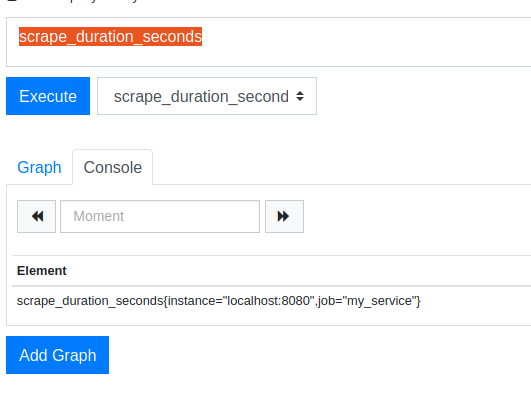
\includegraphics[scale=0.25]{prometheus}
\end{figure}

\end{frame}

\begin{frame}
\frametitle{Prometheus Exporters}

\begin{itemize}
\item Easy\pause
\item Why: Internal\pause
\item Why: Better
\end{itemize}

\end{frame}

\end{document}
